\section{Автоколебания}

\subsection{Автоколебания в системах с одной степенью свободы}
В предыдущих разделах были рассмотрены свободные и вынужденные колебания в диссипативных системах с одной степенью свободы, подчиняющихся дифференциальным уравнениям второго порядка вида \chaptereqref{2.5} и \chaptereqref{2.45} соответственно. Диссипация энергии, обусловленная наличием резистивных элементов в этих системах, в первом случае приводила к затуханию колебаний, а во втором~--- компенсировалась энергией, поступающей от
внешнего источника синусоидального напряжения (или тока). Однако колебания в системе с одной степенью свободы при определённых условиях можно поддерживать, используя постоянный (не синусоидальный) источник энергии, который периодически компенсирует потери колебательной энергии по входящей в систему цепи обратной связи. Такие системы называются \important{автоколебательными}, а протекающие в них процессы~--- \important{автоколебаниями.} Форма и период автоколебаний определяются свойствами самой системы, чем автоколебания существенно отличаются от колебаний вынужденных.

Для определения условий возбуждения автоколебаний в диссипативной системе с одной степенью свободы запишем уравнение \chaptereqref{2.5} с учётом формул \chaptereqref{2.2}, \chaptereqref{2.3} в виде
\begin{equation}
	\eqmark{auto-1}
	\frac{dW}{dt}=-P(t),
\end{equation}
где $W={LI^2}/{2}\;+{q^2}/{2C}$~--- энергия, запасённая в колебательном контуре, а $P(t)=R{{I}^{2}}(t)$~--- мощность потерь. Интегрируя уравнение \eqref{auto-1} по периоду колебаний $T$, приходим к равенству
\begin{equation}
	\eqmark{auto-2}
	W=W_0-\int\limits_{0}^{T}P(t)dt,
\end{equation}
где $W_0$~---~энергия системы в некоторый момент времени, принятый за начало отсчёта периода колебаний $T$. В обычной~--- диссипативной~--- системе $P(t)>0$, так что автоколебания невозможны. Если же мощность потерь $P(t)=R{{I}^{2}}(t)$ в системе \important{знакопеременна}, то подбором режима работы системы можно обеспечить энергетический баланс:
\begin{equation}
	\eqmark{auto-3}
	\int\limits_{0}^{T}{R{{I}^{2}}(t)dt}=0,
\end{equation}
и, следовательно, возбудить в системе автоколебания.

Выполнение условия \eqref{auto-3} возможно, например, в \important{нелинейной} колебательной системе, в которой сопротивление $R$ является функцией тока: $R=R(I)$, причём~--- \important{знакопеременной}. Необходимым для
автоколебательного режима отрицательным «сопротивлением» ${dV}/{dI}$ на «падающих» участках своих вольт-амперных характеристик $I(V)$, представленных на рис.~\figref{auto-1}, обладают, например, газоразрядная лампа (а) и туннельный диод (б). Обычно характеристики вида~(а) называют $S$-образными, а вида~(б)~---~$N$-образными.

\begin{figure}
	\centering
	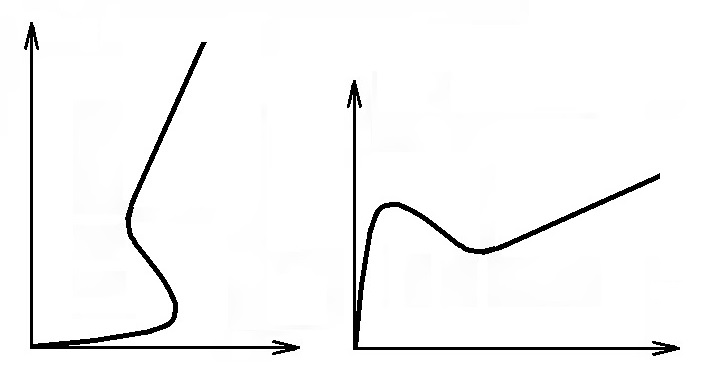
\includegraphics[width=0.9\linewidth]{Chapter_2/auto-1.jpeg}
	\caption{Вольт-амперные характеристики с «падающими» участками:	а) $S$-образным, б) $N$-образным}
	\figmark{auto-1}
\end{figure}

Форма автоколебаний зависит от добротности колебательного контура. При большой добротности характер протекающих процессов почти не изменяется по сравнению с тем, как они протекали бы в системе без поступления
энергии от источника: период и форма автоколебаний будут близки к периоду и форме собственных колебаний. Это связано с тем, что в этом случае от постоянного источника поступает энергия, составляющая малую
долю полной энергии колебательной системы. При малой добротности контура (в общем случае~---~колебательной системы) для поддержания колебаний от постоянного источника должна поступать энергия, сопоставимая с энергией колебаний. В этом случае форма автоколебаний может значительно отличаться от синусоидальной. Наконец, в периодической системе, в которой за период автоколебаний теряется вся накопленная энергия, автоколебания становятся \important{релаксационными} и могут по форме очень сильно отличаться от колебаний синусоидальных.

\subsection{Автоколебания в вырожденных колебательных системах}
Автоколебательная система, не содержащая одного из накопителей колебательной энергии, называется \important{вырожденной}. Колебания в такой системе описываются дифференциальным уравнением первого порядка и, очевидно, могут быть только релаксационными. В рассматриваемом здесь случае электрических колебаний речь идёт об отсутствии в системе одного из реактивных элементов: индуктивности или ёмкости.

В качестве примера рассмотрим представленную на рис.~\figref{auto-2} и рис.~\figref{auto-3} вырожденную колебательную систему, содержащую источник постоянного напряжения $U$, ёмкость $C$, сопротивление $R$ и нелинейный элемент с $S$-образной вольт-амперной характеристикой $I_S(V)$. Как видно, в системе отсутствует второй накопитель колебательной энергии~---~индуктивность.

\begin{figure}
	\centering
	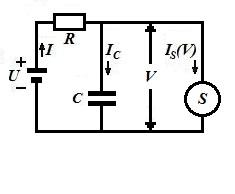
\includegraphics{Chapter_2/auto-2.jpeg}
	\caption{Схема автоколебательной $RC$-системы}
	\figmark{auto-2}
\end{figure}

\begin{figure}
	\centering
	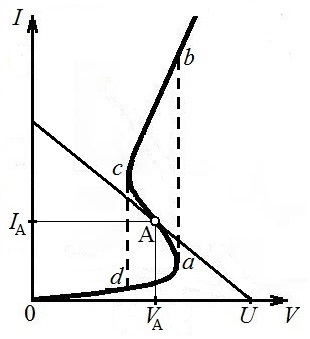
\includegraphics{Chapter_2/auto-3.jpeg}
	\caption{Вольт-амперная характеристика и нагрузочная прямая}						\figmark{auto-3}
\end{figure}

%Рис. 12(а, б). Вырожденная автоколебательная система

Уравнения, описывающие поведение этой системы релаксационного типа,
имеют вид:
\begin{equation} 
	\eqmark{auto-4}
	RI+V=U,~ I=I_C+I_S,~ I_C=C\frac{dV}{dt}, I_S=I_S\left( V \right). 
\end{equation}
Следовательно,
\begin{equation} 
	\eqmark{auto-5}
	RC\frac{dV}{dt}=U-V-R{{I}_{S}}\left( V \right).
\end{equation}

В стационарном состоянии, когда $dV / dt = 0$, должно выполняться равенство
\begin{equation}
	\eqmark{auto-6}
	I_S(V)=(U-V)/R 
\end{equation}
Правая часть здесь представляет \important{нагрузочную} прямую, точки пересечения которой с вольт-амперной характеристикой ${{I}_{S}}\left( V \right)$ определяют стационарные состояния системы. На рис.~\figref{auto-3} параметры $U$ и $R$ выбраны так, чтобы стационарное состояние $A(V_A,~I_A)$ лежало на падающей ветви вольт-амперной характеристики, где, как говорилось выше, возможен
автоколебательный режим. Покажем, что состояние $I_A=I(V_A)$ может быть \important{неустойчивым}. Для этого дадим малое приращение $v$ переменной $V$ в точке
$V_A$ и представим в линейном приближении по $v$ вольт-амперную характеристику $I(V)$ вблизи стационарного состояния $V_A$:
\begin{equation} 
	\eqmark{auto-7}
	I(V)=I(V_A + v)\approx I\left( V_A \right)+{I}'\left( V_A \right)v, 
\end{equation}
где «штрих» означает производную по $V$. Подстановка этого выражения в \eqref{auto-5} приводит к уравнению
\begin{equation} 
	\eqmark{auto-8}
	RC\frac{dv}{dt}=-\left[ 1+R{I}'\left( V_A \right) \right]v, 
\end{equation}
из которого следует, что при условии
\begin{equation} 
	\eqmark{auto-9}
	I'\left( V_A \right) <- {1}/{R}
\end{equation}
возмущение $v$ со временем экспоненциально нарастает, и, значит, стационарное состояние $I_A=I(V_A)$ является неустойчивым. Система при этом будет совершать \important{релаксационные автоколебания}, замкнутая фазовая траектория которых на рис.~\figref{auto-3} состоит из плавных участков $da$ и $bc$ вольт-амперной характеристики между напряжениями $V_1$ и $V_2$, соединённых двумя вертикальными участками $ab$ и $cd$, показанными на рисунке штриховыми линиями. Формально вертикальные участки соответствуют \important{скачкам тока}, которые возможны только при отсутствии индуктивностей в системе, исходно заложенной в данной идеализированной модели. Учёт малой «паразитной» индуктивности элементов схемы, приводящей к появлению э.д.с. индукции и, соответственно, к конечной скорости скачков, добавляет ещё одно дифференциальное уравнение первого порядка. Систему в целом теперь описывает дифференциальное уравнение второго порядка, которое позволяет получить периодическое решение, представляющее автоколебательный процесс.